\documentclass[a4paper,12pt]{report}
\usepackage{color}
\usepackage{graphicx}
\usepackage{subfig}
\usepackage{listings}
\usepackage{media9}
\usepackage{hyperref}

\definecolor{dkgreen}{rgb}{0,0.6,0}
\definecolor{gray}{rgb}{0.5,0.5,0.5}
\definecolor{mauve}{rgb}{0.58,0,0.82}

\begin{document}

\title{CSC190 Notes}
\author{Aman Bhargava}
\date{January-April 2019}
\maketitle

\tableofcontents

\section{Introduction and Course Information}
\begin{itemize}
\item Professor: John Mathai
\item Course: Engineering Science
\item Term: 2019 Spring
\end{itemize}

\chapter{Efficiency and Complexity}
There are two things that effect efficiency of a computer algorithm.
\begin{itemize}
\item Space Complexity = cost in terms of memory
\item Time Complexity = cost in terms of steps
\end{itemize}

\section{Ideal vs. Real Computers}
\begin{tabular}{l|l}
Ideal & Real \\
\hline
Automaton + Workbook & Microprocessor + Memory \\
Mathematical Algorithms & Programs (Sea of Functions) \\
Abstract Data Types & Data Structure 
\end{tabular}

\texttt{Note: ADTs are Abstract Data Types}

Stack is used by C for temporary variables made by functions. Heap is used by CPU and by malloc. All stuff pushed to the stack by a function is freed when the function exits. 

\section{The RAM Model of Computation}
Stands for Random Access Machine Model.
Each simple operation takes 1 time step. Each memory access takes 1 time step. It's actually a really good models for how computers perform.

\subsection{Big Oh Notation}
Usually used for worst case scenarios.
\begin{itemize}
\item $O(g(n))$ is for upper bound of time complexity.
\item $\Omega(g(n))$ is for lower bound of time complexity.
\item $\Theta(g(n))$ is for upper AND lower bound (separated by only a constant)
\end{itemize}

\subsubsection{Dominance Classes}
One class of algorithms in big Oh notation is said to dominate another if their time complexity grows faster than the other.
\begin{enumerate}
\item Linear
\item Logarithmic
\item Linear
\item Super Linear ($n log(n)$)
\item Quadratic
\item Cubic
\item Exponential
\item Factorial
\end{enumerate}
	

\chapter{List ADT implementation in C}
\begin{itemize}
\item An array with length L and end index 'end'
\end{itemize}

\section{Stacks and Queues}
\subsection{Stacks}
\begin{itemize}
\item First in, last out
\item push and pop
\end{itemize}
\subsection{Queues}
\begin{itemize}
\item First in, first out
\item enqueue, dequeue
\end{itemize}

\subsection{Stack and Heap in C}


\chapter{Trees}
\section{Types of General Traversal:}
\subsubsection{Breadth-First Traversal: }
In which you read (1) right to left (2) top to bottom.
\subsubsection{Depth-First Traversal: }
In which you read (1) top to bottom (2) right to left

\subsection{Using Stacks and Queues for Traversals}
\paragraph{Remember: } Stacks $\to$ Depth-First. Queues $\to$ Breadth-First. 
\paragraph{How does it work?}
On inspection, you would think that recursion is the only way to effectively traverse a tree in a depth/breadth-first manner in an easy way. However, you can employ stacks and queues to do this iteritavely. Here are the steps:
\begin{enumerate}
\item Add the root node to the {stack, queue} per the above statement.
\item Pop/dequeue the dequeueing point and print it. Add its children to the {stack, queue}
\item Repeat step 2 until finished. 
\end{enumerate}
This isn't immediately intuitive, but it holds true. Try this on a tree on paper to convince yourself! It's a really cool property of trees/stacks/queues :)

\section{Binary Trees: }
\subsection{Mathai's Weird Definition for Binary Trees vs. Normal Trees}
The rule: The first child of a node goes as the left child in the binary tree. All of its siblings are added as RIGHT children of that first child. Etc.
\subsection{Binary Search Trees: }
Think about the binary search algorithm. The rule is simple: Start with the first node. If the thing you want to add is greater than that node, you add it to the RIGHT child tree. Otherwise, you add it to the LEFT child tree. The rule is recursive and super elegant.
\subsection{Advantages/Disadvantages of Binary Search Trees: }
\begin{enumerate}
\item Advantage: Will (generally) change search from O(n) to O(log(n)) because you only need to visit every LEVEL instead of every NODE (\#levels = log(\#nodes))
\item Disadvantage: If it's not a balanced tree, you could end up with a BST that has \#levels = \#nodes
\end{enumerate}

\subsection{Binary Tree Traversals}
\begin{enumerate}
\item Pre-Order: NLR
\item Post-Order: LRN
\item In-Order: LNR
\end{enumerate}
\paragraph{Mnemonic: } The 'pre'/'post'/'in' refers to the placement of the NODE between/in front of/after the L and R node.

\section{Self-Balancing BST's (AVL Trees): }
The general way we balance binary search trees is with \textbf{rotations}
\paragraph{Level of imbalance: } calculated as nR (number of levels on the right side of the node) minus nL.
\paragraph{Printing Binary Trees in Order: } When you print the left subtree first, then the node, then the right subtree (recursively)
\subsubsection{Types of Rotation: }
\begin{enumerate}
\item Left
\item Right
\item Major Left / Minor Right
\item Major Right / Minor Left
\end{enumerate}

\subsection{Right Rotation: }
The left child becomes the head. The left child's parent (the root) becomes the right child, and the left child of the left child becomes maintains its relationship with the left child of the root. The original left child's RIGHT child becomes the left child of the original root. 
\paragraph{When to do this? } whenever nL - nR $\geq$ 2

\subsection{Left Rotation: }
The right child becomes the head. The right child's parent (the root) becomes the left child, and the right vhild of the right child maintains its relationship with the right child of the original root. The original right child's LEFT child becomes the right child of the original root. 

\subsection{Major Right / Minor Left: }
\paragraph{When to do this: } Whenever the balance on the root and the balance on a subtree is opposite, and the absolute balance of the root is greater than or equal to 2. Tl;dr: You want the subtrees to have the same SIGN of balance as the root node before you do big switches. Condition for doing compelex switches is: balance (root) >=2, sign balance (sub-node) doesn't equal the sign balance (root node)

\subsection{Summary of Tree Rotations: }
\begin{enumerate}
\item For easy, child-free lines to the right and left (root balance = +-2, child banace = +-1 with same sign), use the corresponding rotation to make them triangle trees.
\item For bent ones with root balance = +-2 and child balance +-1 of opposite sign), use minor rotation to get back to case 1 and do a major rotation on the root. 
\end{enumerate}

\begin{figure}[h]
\centering
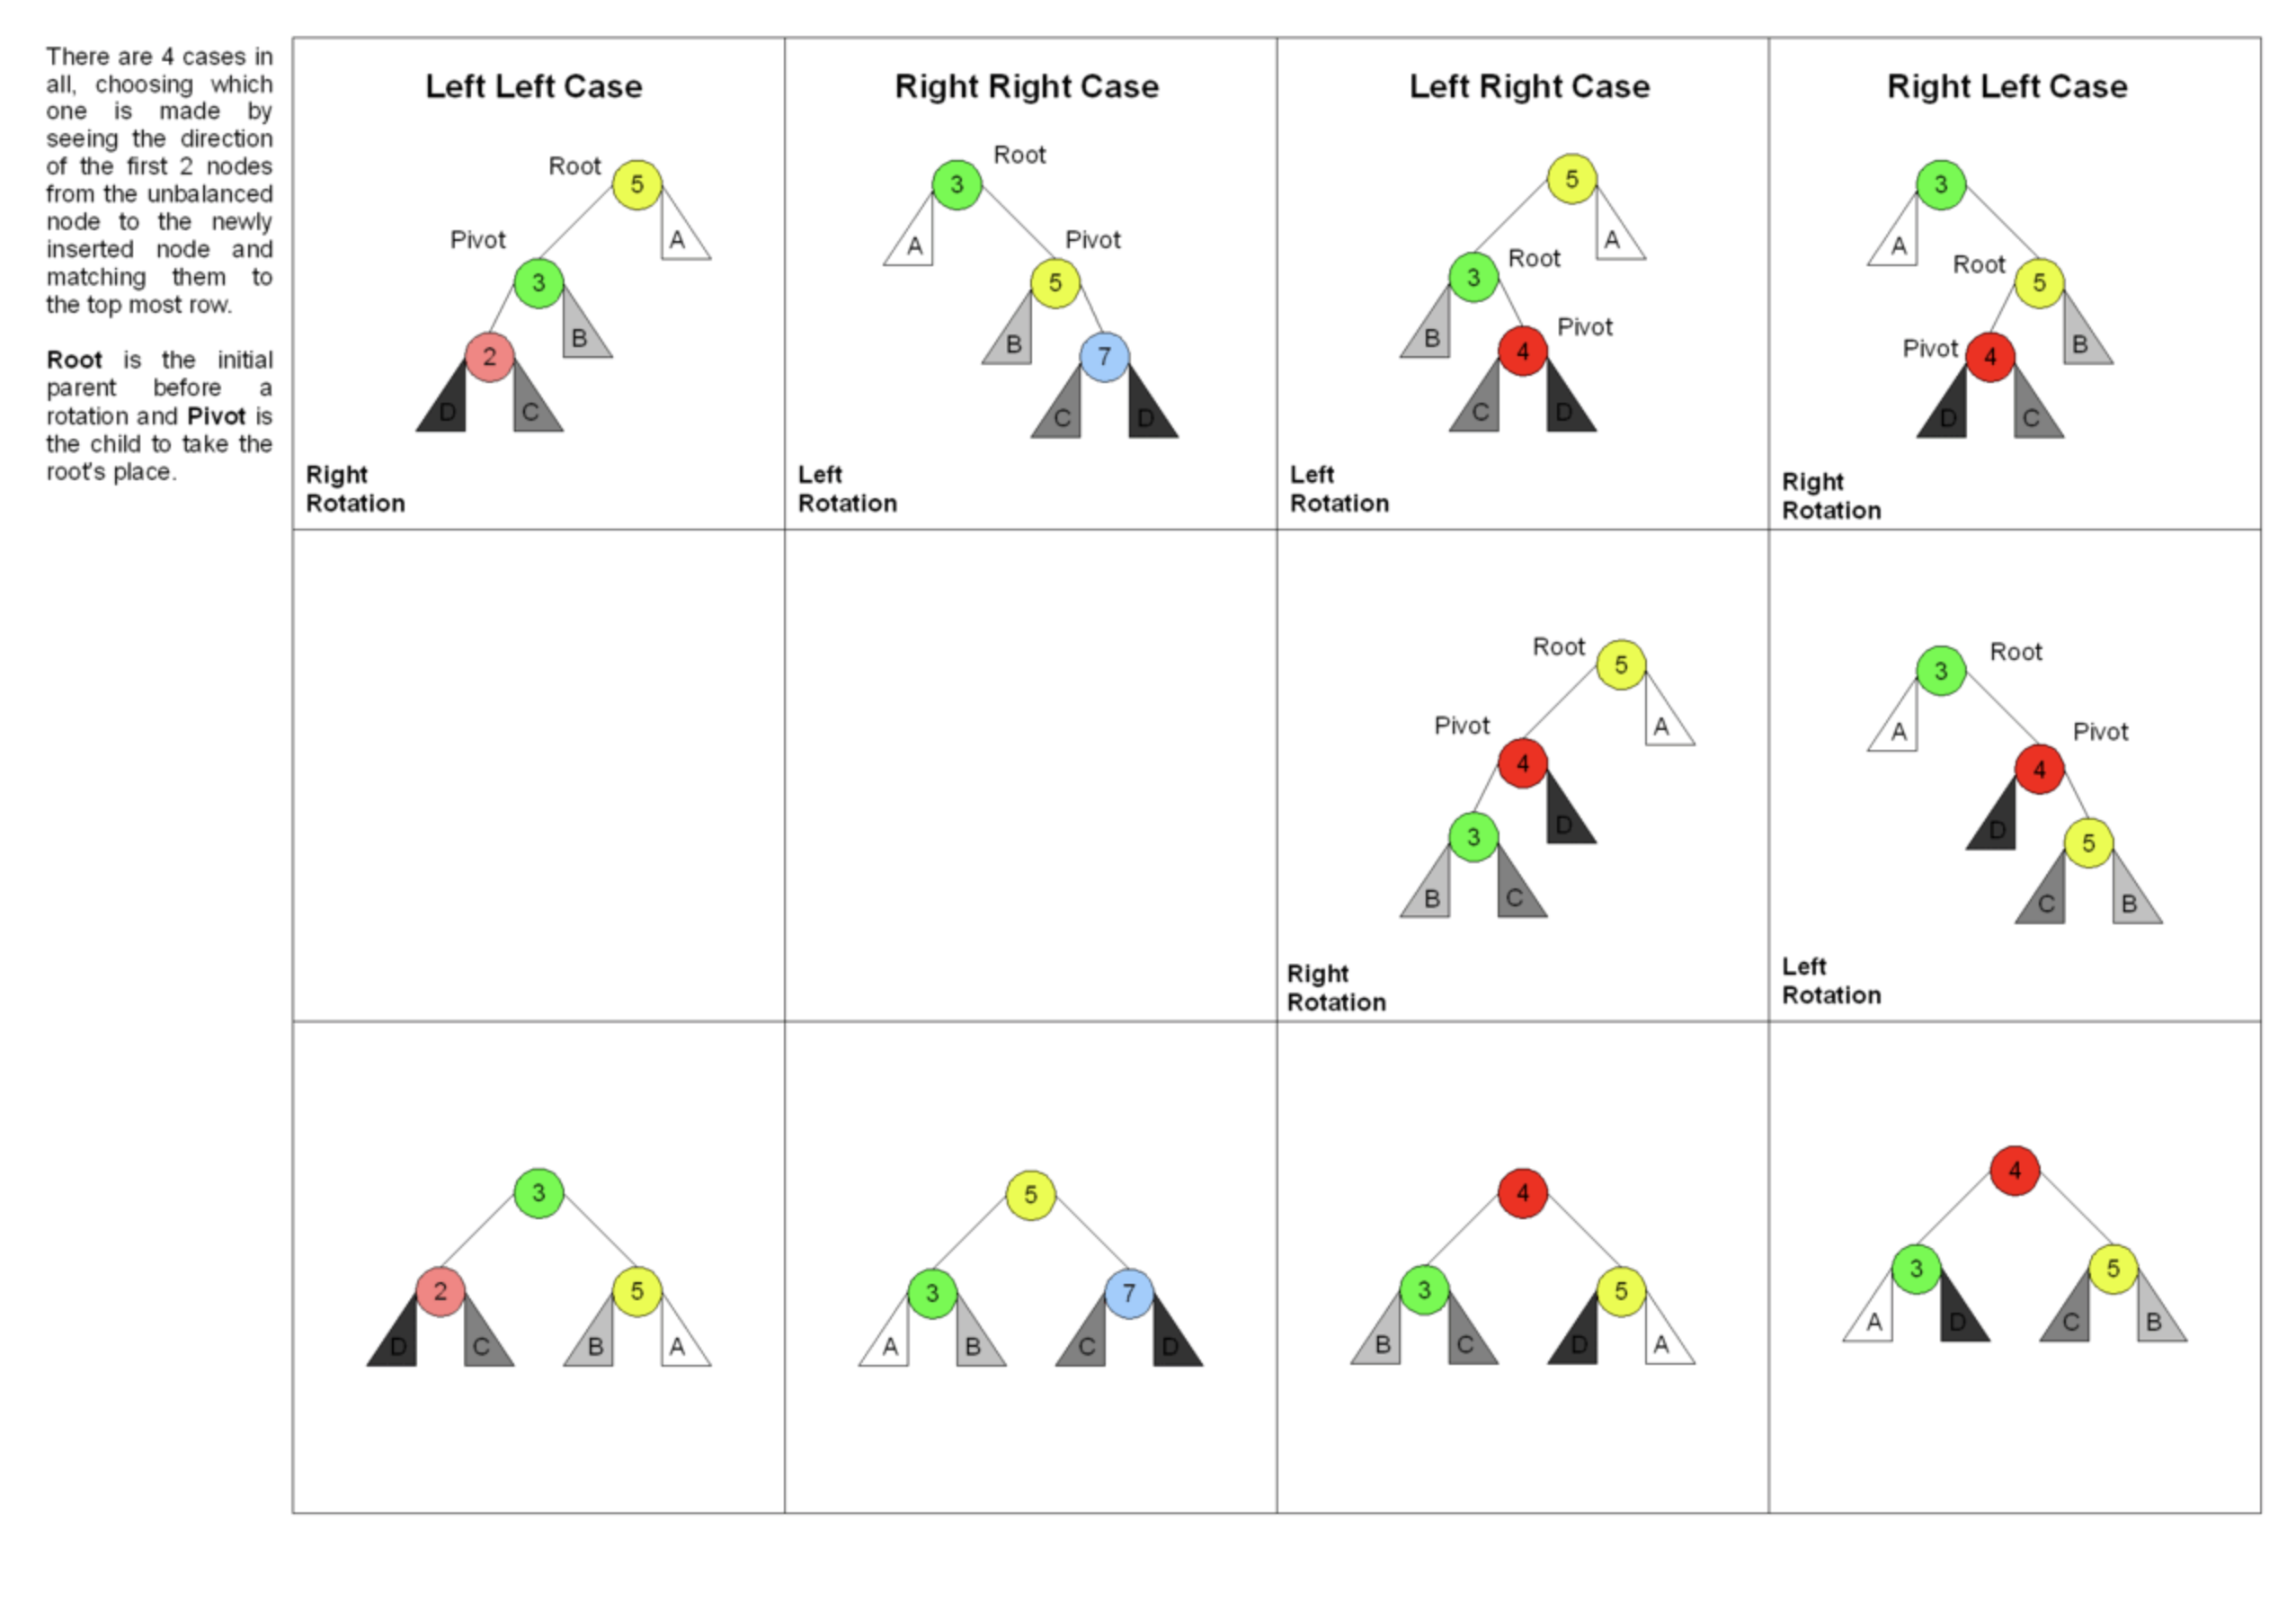
\includegraphics[width=1\textwidth]{media/tree-rotation-summary.png}
\caption{Summary of All Rotation Types}
\label{Tree Rotation Summary}
\end{figure}


\begin{figure}%
    \centering
    \subfloat[label 1]{{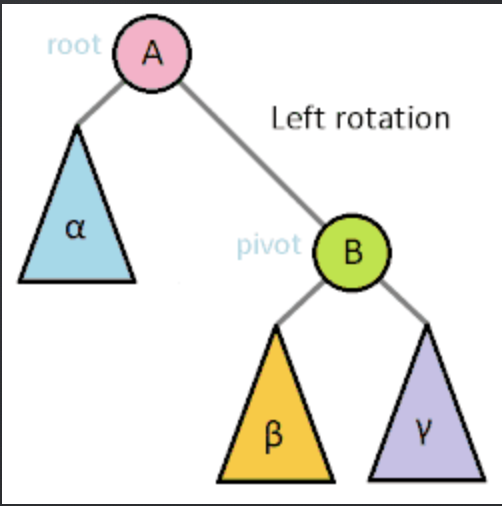
\includegraphics[width=5cm]{media/left-rotation-1.png} }}%
    \qquad
    \subfloat[label 2]{{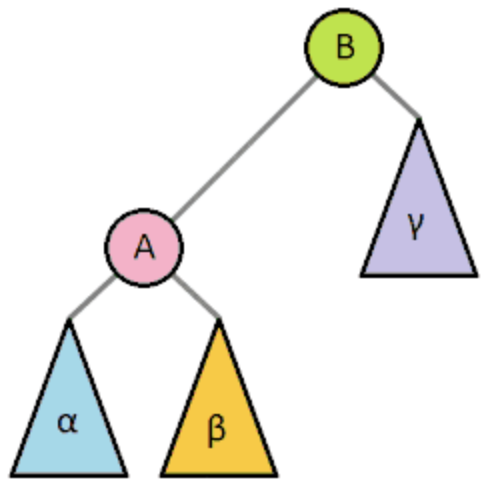
\includegraphics[width=5cm]{media/left-rotation-2.png} }}%
    \caption{Visual Representation of a Left Rotation}%
    \label{fig:example}%
\end{figure}


\begin{figure}%
    \centering
    \subfloat[label 1]{{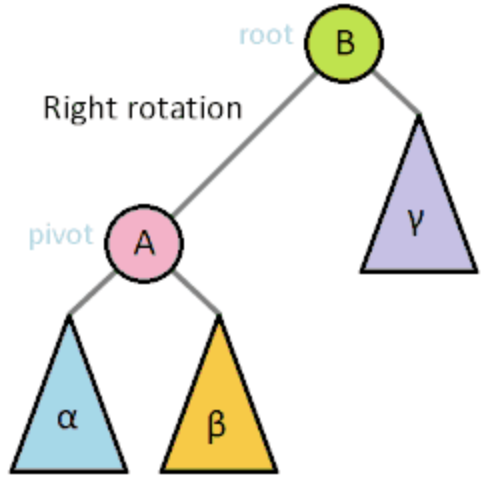
\includegraphics[width=5cm]{media/right-rotation-1.png} }}%
    \qquad
    \subfloat[label 2]{{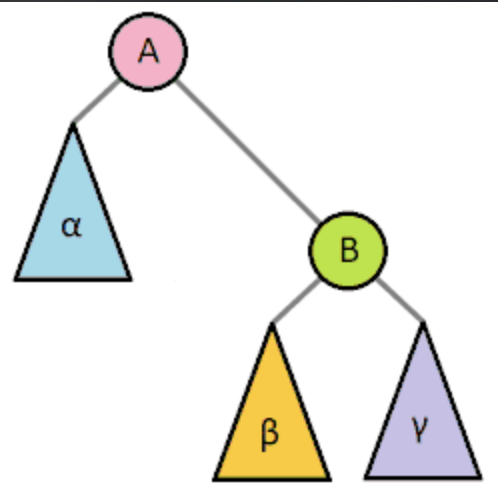
\includegraphics[width=5cm]{media/right-rotation-2.png} }}%
    \caption{Visual Representation of a Right Rotation}%
    \label{fig:example}%
\end{figure}

\subsection{Inserting to a Binary Tree}
\begin{enumerate}
\item If we are passed a pointer to a NULL pointer, then add this info as the NULL pointer.
\item If we are passed a node:
\item Add to the left subtree if we are smaller than that particular node.
\item Add to the right subtree otherwise.
\end{enumerate}


\subsection{Deleting from a Binary Tree}
Swap the node you need to delete with the left child's furthest right child. Then delete the initial node. Also works with the right child's firthest left descendant. Think about how repeated elements might change this up. 

\section{AVL Tree}
AVL trees are self-balancing BST's.
\subsection{When to use which rotation/HOW TO BALANCE: }
Lines of two and zigzags of two are the worst case scenario and they're all you'll ever really have to deal with.
Always do rotations on things that have +/- 2. 

\subsection{Adding to AVL Trees: }
Do binary insert. Then balance it. 

\subsection{Deleting from AVL Trees: }
Do binary deletion. Then balance it.

\section{Priority Queues}
Operations:
\begin{enumerate}
\item Insert element
\item Find minimum
\item Find maximum
\end{enumerate}

The queue can be an ordered list, unordered list, binary search tree, and more. 

\section{Hashes and Strings}
Hashes = way to maintain a dictionary. Takes advantage of $O(1)$ complexity of finding something once you know its key (location) in a list/array. 

\paragraph{Example: } indexing strings. Hash function uses each letter as a number in a base-alphabet number system. Then you map any string to unimaginably large numbers. To find where they should go in an array, take the output \% the size of the array.

\paragraph{Problem: } you're likely to have some collisions in terms of where you assigned a string. Let $m$ be the length of the array. 

\paragraph{Solution 1: Chaining } where you have linked lists for each hash table entry that has multiple items hashing to it. But this uses a lot of memory for pointers.

\paragraph{Solution 2: Open Addressiong } where you just chuck it in the next sequentially available slot. It's not great though because repeated deletion and addition may result in an entirely random hash table.  

\section{Heap}
Max heap = top heavy. Min heap = bottom heavy.
\subsection{Implementation as List (0-indexed)}
\begin{enumerate}
\item Child 1 Index = Parent Index*2 + 1
\item Parent Index = (Child Index-1) // 2
\end{enumerate}

\subsection{Adding to a Heap}
\begin{enumerate}
\item Add to the last element in the heap/list
\item If parent and child relationship is OK, then stop.
\item Otherwise, swap and go back to step 2.
\end{enumerate}

\subsection{Deleting from Heap}
\begin{enumerate}
\item Replace deleted item with the item furthest down and to the right in the heap.
\item Heapify by swapping with parent if necessary or with child if necessary.
\end{enumerate}

\subsection{Searching a Heap}
You have to search everything. But you can stop if you reach something larger (in the case of a min heap) or smaller (in the case of a max heap). 

\chapter{Graphs}
\paragraph{What's a graph? } Bunch of nodes with connections (verticies and edge). Each connection/edge can have a weight. Connections/edges can either be directional or non-directional. The path length between two is the sum of the weights of the edges that you traverse to get there. 

$$G = (V, E)$$
Graph is made of a set of verticies ($V$) connected by set of edges ($E$).

\paragraph{What about notation? } $E_{a \to b}$ connects a to b. If it's non-directional, then $E_{b \to a}$ is therefore valid and existent. However, if it is a directional edge, then it does not necessary exist.

\section{Types of Graphs}
\begin{enumerate}
\item Weighted and unweighted graphs (verticies can have weight)
\item Directed vs. undirected graphs
\end{enumerate}

\subsection{Paths}
A set of connected edges and nodes that leads from one node to another.

\subsection{Cycles}
A path that leads back to where it started without using any edges twice. Must use an edge.

\subsection{Strength of Connections}
If $A \to B$ in a non-directional way, it is a strong connection. However, if $A \to B$ is directional, it is considerred weak. Also, if it is indirectly connected, it doesn't affect the strength of the connection.

\subsection{Articulation Vertex}
A vertex that, if removed, will change the connectivity of other verticies.

\section{Traversal of Graph: Prim's Algorithm}
\paragraph{What it does: } finds a minimum spanning tree. It's a greedy algorithm (i.e. it takes the locally optimal path at each point). It always converges to an optimal solution, but that's rare for greedy algorithms. 

\paragraph{Steps in Prim's Algorithm: }
\begin{enumerate}
\item Start with a vertex chosen at random.
\item Choose the minimally-weighted edge that's connected to that (set of) vertex.
\item Add the vertex connected by that minimally-weighted edge to the minimum spanning tree.
\item Now repeat steps 2-3 with the new set of vertices until you get the minimum spanning tree.
\end{enumerate}

\paragraph{Topological Ordering in a Graph}
All about finding an "order" to a graph (e.g. pre-requisite courses represented with directed edges).

You can only find topological ordering for some graphs. They must be \textbf{directed} and \textbf{acyclic} (i.e. \textbf{DAG} graphs).

\paragraph{For the courses example:}
\begin{itemize}
\item If you don't need any pre-requisite (i.e. no traversal from start is needed), it has \textit{in-degree} of 0.
\end{itemize}

\section{Representations of Graphs: Adjacency Matrices}
\begin{itemize}
\item $n \times n$ matrix
\item If $A+{ij}$ is non-zero value $a$ then vertex $i$ is connected to $j$ with weight $a$
\end{itemize}

\section{Dijkstra's Algorithm: Pathfinding}
Here are the steps to run this algorithm by hand:
\begin{enumerate}
\item Start with a set of visited nodes, unvisited nodes, and a set of tentative weights all set to infinity (except for the starting node)
\item At each step, see what the minimum distance from each visited node to its neighbour is. If the total distance from the starting node is less than the tentative weight currently says, update the weight.
\item Continue updating the tentative weights and the set of visited/unvisited nodes, along with the paths needed to get to each node.
\end{enumerate}

\paragraph{Complexity of the Algorithm}
Time complexity: $O(n^2)$ (worst case, discussed in textbook)



\chapter{Bit Manipulation}
Have you ever wanted to be a cool computer person who does things with ones and zero's instead of actual letters and numbers like a normal person? If so, this is the right chapter for you!

\section{Converting to and from Different Bases}
Base 10, 2, and 16 are most commonly used. Base 16 is just a way to read base 2 in a more efficient manner. In order to work with bits it's pretty important to know how to convert back and forth because the test is all on paper. 

\subsection{Converting from base 10 $\to$ base 2}
You keep dividing by two, keeping track of the remainder. Eventually the number you will be trying to divide by two will be 1. You keep going until it's zero + remainder(1). Then you read the reaminders upward from that final 1.

\subsection{Converting from base 2 $\to$ base 16}
Any hex number can be expressed as 4 binary digits. Make a correspondence table between quadruplets of binary numbers and hex (1-f, inclusive). To convert to base 16 subdivide from right to left in groups of four binary digits. Pad the leftmost part with leading zeros and convert using the table. 

\subsection{Converting from base 10 $\to$ base 16 (and vice versa)}
Just go through base 2 fam.

\section{Bitwise Operators}
\subsection{How to print bits of a variable}
\begin{itemize}
\item printf("\%x\textbackslash n", var1);
\item You usually use unsigned ints and unsigned chars.
\item Unsigned chars are 8 bits (two hex characters, 1 byte). 
\item Unsigned ints are 32 bits (8 hex characters, 4 bytes).  
\item Each hex character represents half a byte.
\item When you print out a low-valued int, it won't necessarily show all 8 hex characters (it eliminates leading zeros).
\end{itemize}

\subsection{Altering Bits}
\begin{enumerate}
\item \& - And operator; Only outputs 1 when both inputs at that bit are 1.
\item $|$ - Or operator; Outputs 1 if at least one of the inputs at that bit are 1. 
\item $\hat{}$ - Exclusive or operator (xor); Outputs one if only one fo the inputs is 1. 
\item \textasciitilde - Not operator; flips the bits (e.g. ~a = opposite of a)
\item $<<$ - shift left operator; shifts all bits left, padding the right in with zeros (e.g. $c = a << 2;$)
\item $>>$ - shift right operator; shifts all bits right, padding left with zeros (e.g. $c = a >> 2;$)
\end{enumerate}

\chapter{Sorting and Searching Algorithms}
Sorting is pretty darn important. You can probably reason out why that is. Here are some of the major sorting algorithms, and below is a table summarizing the time complexity of these algorithms: 

\begin{tabular}{l|l|l|l}
\textbf{Algorithm} & \textbf{Time Complexity} \\
\hline
\textit{} & \textit{Best} & \textit{Average} & \textit{Worst} \\
\hline
Selection Sort & $\Omega(n^2)$ & $\Theta(n^2)$ & $O(n^2)$ \\
Insertion Sort & $\Omega(n)$ & $\Theta(n^2)$ & $O(n^2)$ \\
Bubble Sort & $\Omega(n)$ & $\Theta(n^2)$ & $O(n^2)$ \\
Heap Sort & $\Omega(nlog(n))$ & $\Theta(nlog(n))$ & $O(nlog(n))$ \\
Merge Sort & $\Omega(nlog(n))$ & $\Theta(nlog(n))$ & $O(nlog(n))$ \\
Quick Sort & $\Omega(nlog(n))$ & $\Theta(nlog(n))$ & $O(n^2)$ \\
Radix Sort & $\Omega(nk)$ & $\Theta(nk)$ & $O(nk)$ \\
\hline
\end{tabular}

\section{Selection Sort}
\begin{enumerate}
\item Define start of array as $s = 0$ and $e = len(array)$
\item Find minimum element in array $s \to e$ and swap it with the element at $s$
\item Add 1 to s and repeat step 2 until $s = e$.
\end{enumerate}
\section{Insertion Sort}
\begin{enumerate}
\item The "sorted" partition of the array starts with one element.
\item You then take the next element after the "sorted" partition and insert it into the sorted partition in order.
\item Repeat until the sorted partition is the size of the array.
\end{enumerate}

\section{Bubble Sort}
\begin{enumerate}
\item Go through element 0 to element len(array)-1. If the element is not in order with the element in front of it, switch them.
\item Keep doing this until swapping is no longer necessary.
\end{enumerate}

\section{Heap Sort}
\begin{enumerate}
\item Make a heap out of the array
\item Keep popping the max/min element from the heap and re-heapifying until the heap is empty.
\item You now have a sorted list.
\end{enumerate}

\section{Merge Sort}
\begin{enumerate}
\item Have a function called merge that 'zips' two sorted lists together into one big sorted list (pretty simple if you think about it)
\item Unless the given partition is of length 2 or 1, keep calling the mergesort function on each half of the given partition.
\item If the partition is of length 2, swap them if they're out of order. Otherwise, return the partition.
\item If the partition is of length 1, return the partition.
\item Zip up the two return values from the recursive call of the mergesort algorithm.
\end{enumerate}

\section{Quick Sort}
\subsection{Partition}
This takes a list and 2 inputs including the begin and end index of the section.
\begin{enumerate}
\item The end element is the 'pivot'.
\item You set your 'first high' to the beginning element
\item You go through with a counter i
\item If the thing at 'i' is smaller than the pivot, you swap it with whatever is at 'first high' and add one to 'first high'.
\item Repeat this, then swap the element at 'pivot' with the element at 'first high'
\item Return the index of 'first high'. You just partitioned the list into 2 parts around the pivot.
\end{enumerate}

\subsection{Quick Sort}
\begin{enumerate}
\item Just keep running the partition algorithm recursively, fam.
\end{enumerate}

\section{Radix Sort}
\begin{enumerate}
\item Make k bins where k is equal to the number of potential place valuese (i.e. 10 in base 10)
\item Start by binning based on the lowest place value.
\item Repeat the process with the second lowest place value and so on.
\item Continue until everything is sorted.
\item Runs in $O(nk)$ time where $k$ is the maximum number of place values. 
\end{enumerate}





\end{document}
